\chapter{Experiments}
\label{Experiments}
In experiments \ref{Expt_1} and \ref{Expt_2}, we consider Pix2Pix as an ``upperbound" image translation method, and measure the degree to which the performances of CycleGAN-naive and CycleGAN-balanced approach this upperbound. Pix2Pix is expected to perform better due to its paired (or supervised) training. The GANs systems as well as all the model training are implemented using \textit{PyTorch}. The online experiment tracking tool provided by \textit{Weights and Biases} (abbreviated as \textit{WandB}) is used to record training losses and validation metrics in experiments involving model training (\ref{Expt_1} and \ref{Expt_2})).



%%%%%%%%%%%%%%%%%%%%%%%%%%%%%%%%%%%%%%%%%%%%%%%%%%%%%%%%%%%%%%%%%%%%%%%%%%%%%%%%%%%%%%%%%%%%%%%%%%%%%%%%%%%%%%%%%%%%%%%%%%%%%%%%%%%%%%%%%%%%%%%
\section{Experiment 1: Testing the GANs on Depth Estimation Problem}
\label{Expt_1}

This experiment concerns with testing the GAN systems on the simulated problem of depth estimation from multimodal input comprising of photographic and surface normal images.


% ---------------------------
\subsection{Experiment Setup}

\subsubsection{Training configuration}
The curated dataset for the depth estimation task is a subset of the original ClearGrasp dataset (see \ref{ClearGrasp_Depth_Estimation}). During training, images of all three modalities are first rescaled to size 512$\times$256 and normalized to [-1, 1] range.  In Pix2Pix, $\lambda_{elem}$ value of 100 was observed to produce good results, and $\lambda_{elem}$ value of 10 is used in both CycleGANs. Similar to the optimizer configuration used in the original Pix2Pix and CycleGAN papers \cite{isola2017image, zhu2017unpaired}, we use Adam optimizer with moment parameter settings $\beta_1$=0.5 and $\beta_2$=0.999. An initial learning rate of 0.0002 is used for the generators and 0.0001 for the discriminators. We train each model with a batch size of 1 on full images for 50 epochs. The learning rates are fixed for the first 25 epochs and then linearly decayed to 0 over the next 25 epochs. Model validation is performed after each epoch. The training was run on an NVIDIA Tesla P100 SXM2 (16 GB) GPU hardware provided as part of the RWTH Aachen Compute Cluster, and the training time for Pix2Pix, CycleGAN-naive, and CycleGAN-balanced models was approximately 2 hours, 4 hours, and 5 hours respectively.

\subsubsection{Evaluation settings}
We use pixel-wise mean-squared error (MSE) between the synthetic and ground truth depthmaps as the evaluation metric. Before computing the MSE, the image intensities are converted back to their original depth representation in meters.


% -------------------------------
\subsection{Results and Analysis}
Table \ref{tab:cleargrasp_quant} reports the MSE values for each of the models' predictions on the validation set. Pix2Pix performs the best by a large margin and is also the most robust among the three, as expected, setting the performance upperbound among the three models. CycleGAN-balanced achieves better results as compared to CycleGAN-naive. 

\begin{table}[h!]
    \small
    \centering
    \begin{tabular}{ccccccc}
        \textbf{Method} & \textbf{MSE} \\
        \hline
        Pix2Pix    & \textbf{0.004} $\pm$ 0.005 \\
        CycleGAN-naive    & 0.192 $\pm$ 0.253 \\
        CycleGAN-balanced    & 0.147 $\pm$ 0.170 \\
    \end{tabular}
    \caption{Mean-squared error (expressed in meters$^2$) over the validation subset.}
    \label{tab:cleargrasp_quant}
\end{table}

\begin{figure}[h!]
    \centering
    \makebox[\textwidth][c]
    {   
        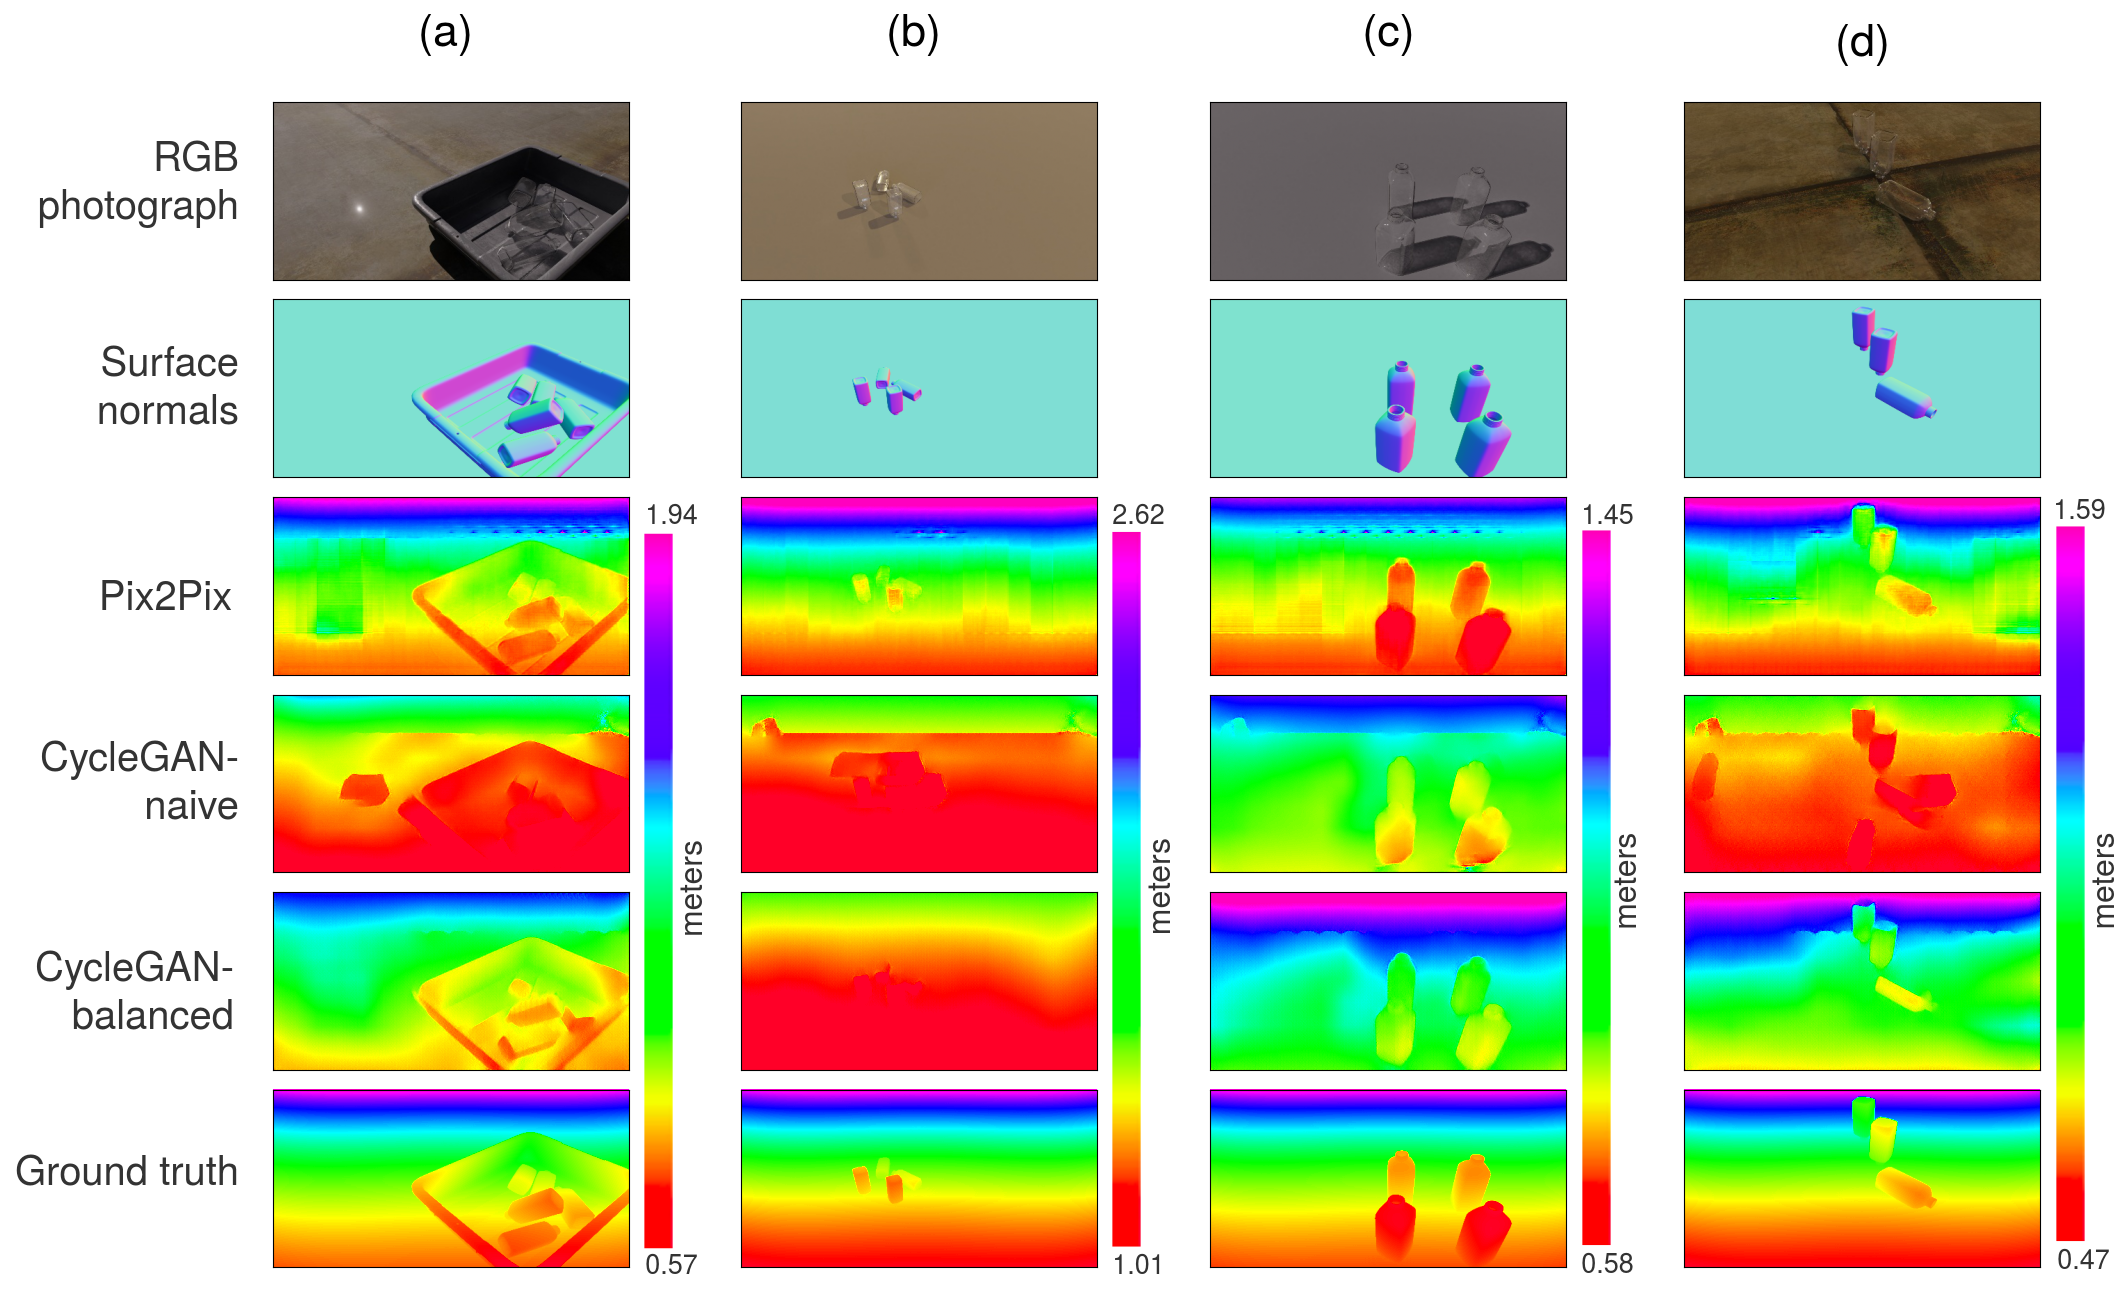
\includegraphics[width=1.05\linewidth]{figures/Expt_1/Cleargrasp_Results-viz.png}
    }
    \caption{Selected validation samples chosen to highlight the challenges in input data –- (a) a nearby tray containing transparent objects and a reflection on the floor, (b) distant objects, (c) objects casting strong shadows, and (d) a strong cross-shaped pattern on the floor. Pix2Pix model estimated the depth of the transparent objects, other objects and the floor very close to the ground truth. CycleGAN-naive produced depthmaps with heavy artifacts, which were absent in case of CycleGAN-balanced, notably in (a) and (d).}
    \label{fig:cleargrasp_qual}
\end{figure}

Figure \ref{fig:cleargrasp_qual} shows qualitative results with samples that are representative of the MSE measurements. In general, Pix2Pix predicts the depthmaps accurately with minimal artifacts. The predictions of CycleGAN-balanced contain heavy artifacts, including horizontal edges that are observed recurring across multiple images at the same position (a sign of mode collapse) and hallucinated spurious objects. The model doesn't learn the concept of depth. In case of CycleGAN-balanced, the predicted depthmaps contain a greatly reduced amount of artifacts. The model appears to have learned to infer depth, although only in a limited manner -- the depth of larger non-transparent objects (such as the tray) is estimated better compared to that of the transparent objects.

\begin{figure}[h!]
    \centering
    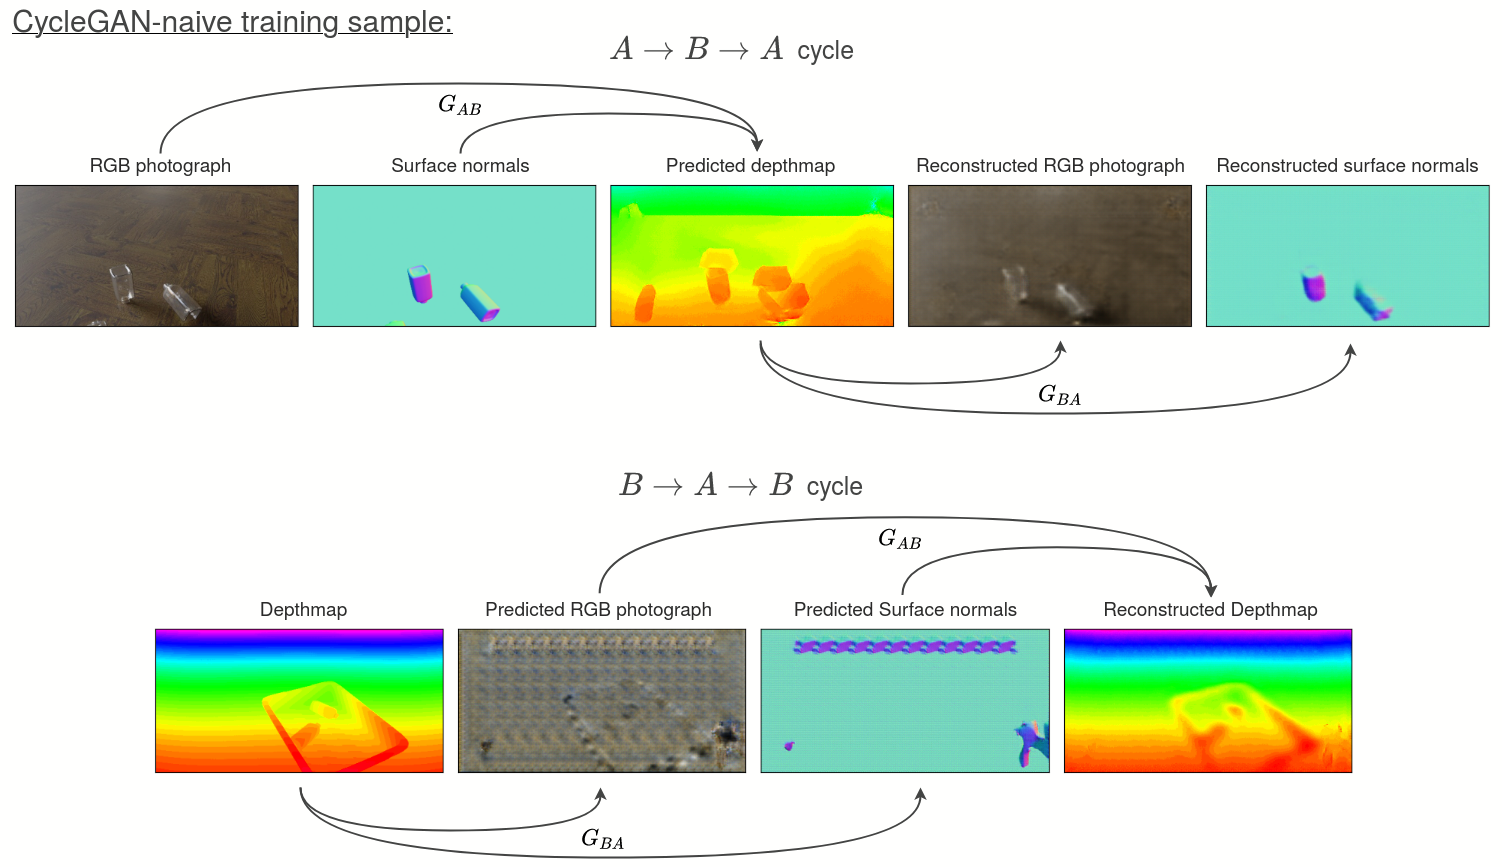
\includegraphics[width=\linewidth]{figures/Expt_1/cyclegan_naive_cycles.png}
    \caption{Single unpaired training sample and generator outputs of the fully-trained CycleGAN-balanced model. In \textit{A}$\rightarrow$\textit{B}$\rightarrow$\textit{A} cycle, $G_{AB}$ predicted depthmap with hallucinated structures and yet $G_{BA}$ is able to recover back the photograph and surface normals from it. Similarly, in the \textit{B}$\rightarrow$\textit{A}$\rightarrow$\textit{B} cycle, the same $G_{BA}$ failed to compute the ``correct" photograph and surface normals from a real depthmap, and yet despite the noisy images it produced, $G_{AB}$ somehow reconstructed the depthmap from them. Here, the training problem is ill-posed and cycle-consistency fails as a result.}
    \label{fig:cleargrasp_cyclegan_naive_cycles}
\end{figure}

\begin{figure}[h!]
    \centering
    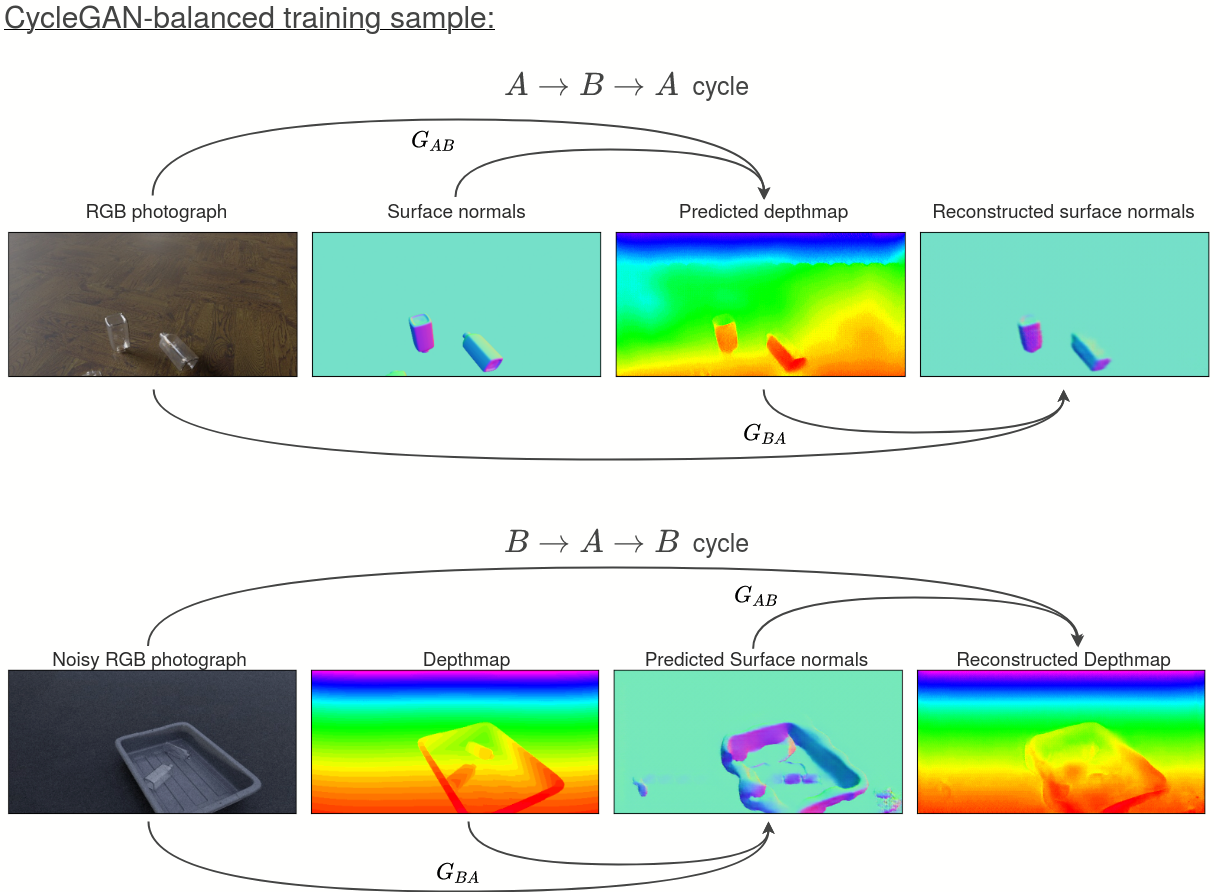
\includegraphics[width=0.8\linewidth]{figures/Expt_1/cyclegan_balanced_cycles.png}
    \caption{Single unpaired training sample and generator outputs of the fully-trained CycleGAN-balanced model. In both cycles, the translation task is mainly across surface normals and depthmaps, while the available photograph serves as a common contextual information for prediction and reconstruction. In \t cycle, the predicted surface normal image has a deformed structure. However, the reconstructed depthmap reflects this distortion and thus the cycle-consistency requirement can act on correcting it. Here, the training problem is well defined and solvable.}
    \label{fig:cleargrasp_cyclegan_balanced_cycles}
\end{figure}

To give a concrete example of the conceptual issues with CycleGAN-naive described earlier in \ref{cyclegan}, the outputs produced by both its generators are visualized and compared with the generator outputs of CycleGAN-balanced. Figures \ref{fig:cleargrasp_cyclegan_naive_cycles} and \ref{fig:cleargrasp_cyclegan_balanced_cycles} show the outputs of the fully-trained CycleGAN-naive and CycleGAN-balanced models, respectively, given an equivalent set of unpaired input images. In Figure \ref{fig:cleargrasp_cyclegan_naive_cycles}, the generator $G_{AB}$ of CycleGAN-naive in the \textit{A}$\rightarrow$\textit{B}$\rightarrow$\textit{A} cycle produces an incorrect depthmap containing spurious objects from the given photographic and surface normal images. $G_{BA}$ then not only uses this flawed depthmap to almost accurately reconstruct the objects in the original photograph and surface normal image, but also manages to perfectly recover the colors in the photograph. In order to satisfy cycle-consistency, $G_{AB}$ would likely have encoded information about the transparent objects' shape as well as the photograph's optical information into the depthmaps, which $G_{BA}$ would have used to almost completely recover the input images, especially the color photograph. The model learns to bypass the content-preservation requirement which cycle-consistency is intended to indirectly encourage. In \textit{B}$\rightarrow$\textit{A}$\rightarrow$\textit{B} cycle, the generator $G_{BA}$, which in previous cycle relied on information encoded in the fake depthmap images, now fails to predict the ``correct" photograph and surface normals given a real (and noise-free) depthmap, thereby producing highly noisy images completely devoid of any meaningful features. However, $G_{AB}$ still reconstructs the depthmap from these noisy images, indicating that the $G_{BA}$ must have encoded relevant information, possibly as noise, into its output. Cycle-consistency is bypassed in this case as well. The problem arises because although the task of learning $G_{AB}$ may have been solvable, learning its inverse ($G_{BA}$) isn't, since such a unique inverse mapping doesn't exist. The learning problem as formulated for the CycleGAN-naive model is ill-posed, in the sense that there is no solution to it, and therefore, the training would fail inevitably. 

On the other hand, the outputs of CycleGAN-balanced generators shown in Figure \ref{fig:cleargrasp_cyclegan_balanced_cycles} highlight the system's improved capability of learning the relevant mappings. Here, the main participant modalities of the translation task are the surface normal image and the depthmap. Neither of the generator tasks involves synthesizing the color photographs from simpler modalities. Using the photographic images always as an input component for the generators provides them shared contextual information within each cycle. Here, the unpaired learning problem for CycleGAN-balanced is better formulated and solvable, and hence the training process can yield a suitable translation model.



%%%%%%%%%%%%%%%%%%%%%%%%%%%%%%%%%%%%%%%%%%%%%%%%%%%%%%%%%%%%%%%%%%%%%%%%%%%%%%%%%%%%%%%%%%%%%%%%%%%%%%%%%%%%%%%%%%%%%%%%%%%%%%%%%%%%%%%%%%%%%%%
\section{Experiment 2: Image Quality Metrics For Synthetic HX4-PET Assessment}
\label{Expt_2}
This experiment focuses on evaluation of the GAN systems for the conditional HX4-PET synthesis task. Global quality of the HX4-PET-syn images is assessed using general metrics of image quality and similarity. Additionally, the applicability of these metrics in tracking model convergence during training is explored.


% ---------------------------
\subsection{Experiment Setup}

\subsubsection{Training configuration}
The dataset used in this experiment is the Maastro Lung HX4-PET dataset after undergoing the preparation steps described in \ref{Data_Processing}. The patch-based training pipeline described in \ref{training_pipeline} is used for all model training. Because a the models are trained on sets of patches extracted from the images using stochastic strategies, the notion of an ``epoch" doesn't exist here. Instead, the number of iterations is used as a measure of training duration, where an iteration is composed of sampling a set of image patches from the full images, performing the required forward passes through the networks, and updating the weights of all the networks in the GAN system. We train each GAN model for 60,000 iterations. The scaling factor $\lambda_{elem}$ for the element-wise loss in Pix2Pix is set to 10, and a $\lambda_{cyc}$ of 10 is used for the cycle-consistency loss in the CycleGANs. Similar to experiment \ref{Expt_1}, Adam optimizer is used with settings $\beta_1$=0.5 and $\beta_2$=0.999. Initial learning rates 0.0002 for the generators and 0.0001 for the discriminators are used during the first 30,000 iterations followed by linearly decaying the learning rate values to 0 over the remaining 30,000 iterations. Model validation is performed every 1000 iterations. All models are trained with batch size 1.

Training was performed on an NVIDIA Tesla V100 SXM2 (32 GB) GPU provided by Data Science Research Infrastructure (DSRI) \footnote{\url{https://maastrichtu-ids.github.io/dsri-documentation/}} of Maastricht University. The 3D training of the Pix2Pix, CycleGAN-naive, and CycleGAN-balanced models took 9.5 hours, 13 hours, and 15.25 hours, respectively. 


\subsubsection{Evaluation settings}
The set of six image quality and similarity metrics described in \ref{image_quality_metrics} are used to assess the quality of HX4-PET-syn images, given the corresponding ground truth HX4-PET-reg images. The intensity scale is divided into 100 bins while computing NMI (for entropy calculation) and global histogram distance.

Additionally, a systematic visual inspection of the synthetic images is performed to identify failure modes that are typical to each GAN model. This would also enable validating the assessment of the image quality metrics. For each patient in the validation set, each model's predicted HX4-PET-syn images were visualized and inspected along all three axes -- axial, sagittal and coronal -- using the \textit{3D Slicer} visualization software under a window of [0, 1.3] SUV. This window is chosen so that the most of the variation in image intensities could be covered. The following set of image degradation criteria are defined to guide the visual inspection:

\begin{enumerate}
    \item \textit{Presence of background noise patterns:} It is well known that checkerboard artifacts can occur in GAN generated images usually due to the the nature of the transposed convolution operation used in upsampling layers \cite{odena2016deconvolution}. This criterion aims at judging the images based on the presence of such periodic noise patterns in the region outside the body where the hypoxia signal is supposed to be zero. This criterion would be satisfied only when severe amount of noise is present such that it is readily visible to the observer in most slices along all three axes of the 3D image.
    
    \item \textit{Presence of noise patterns in the body region:} Checkerboard and other periodic noise patterns in the background may be absent in better performing models because all models were trained on body-masked images whose background intensities were set to zero signal value (0 SUV in PET and -1024 HU (air) in CT). Regardless, such noise can also possibly occur \textit{within} the body region, i.e. the foreground of the image. This criterion aims to account for this, and to satisfy it the noise must be severe enough to be easily detectable by the observer, must be wide spread in roughly the central parts of the body area (i.e. away from boundary regions) and recurring across multiple slices along all three image axes. 
    
    \item \textit{Presence of hallucinated structures:} Generated scans can possibly contain structures which wouldn't be characteristic of human physiology, which might have been constructed by the model to increase the resemblance of the image to the target distribution samples. Many of such structures could be conspicuous enough to be noticeable to non-experts, however others would be too challenging even for trained professionals to discover. This is because unlike CT which shows anatomical structure in high detail, PET images, and especially HX4-PET, show only vague and diffused forms. The synthetic HX4-PET is bound to have at least some differences in these forms as compared to the ground truth, and therefore it is difficult to draw a line past which the differences can be deemed a hallucinated object. Hence, this criterion focuses on the former, more conspicuous, type of artificial structures. For example, isolated high-intensity objects with globular or ring-like shape, similar to common tumor hypoxia signatures, in regions where they shouldn't exist. Using the ground truth as reference, detection of even a single such structure in a predicted image would satisfy this criterion.
    
    \item \textit{Breaks in the existing structure:} Abrupt breaks in structure, for example, holes and gaps with sharp edges, inside the patient's body region in the generated images can occur when the model has not learned relevant anatomical features. Many such glitches can be easily detected by an untrained observer, and this criterion aims to account for their presence in the synthetic HX4-PET images. One or more severe gaps of such type in the image foreground would satisfy this criterion.
\end{enumerate}



% ------------------------------------------------------------------
\subsection{Results and Analysis 1: Evaluating Fully Trained Models}
Performance of the three 3D models as measured by the six image metrics is reported in Table \ref{tab:hx4_image_quality_quant}. Pix2Pix emerges to be the best performing model as evaluated by all six metrics, followed by CycleGAN-balanced whose performance values are very close to those of Pix2Pix. CycleGAN-naive performs the worst, as agreed by all the metrics. Borda counting based on the individual performance rankings of the metrics resulted in the same global ranking on the models -- Pix2Pix as the best model, followed by CycleGAN-balanced and then finally CycleGAN-naive.

% % Original table
% \begin{table}[h!]
%     \scriptsize
%     \centering
%     \makebox[\textwidth][c]
%     {
%         \begin{tabular}{ccccccc}
%             \textbf{Method}   & \textbf{MSE}   & \textbf{MAE}   & \textbf{PSNR}   & \textbf{SSIM}   & \textbf{NMI}   & \textbf{Histogram dist.} \\
%             \hline
%             Pix2Pix   & \textbf{0.009} $\pm$ 0.006   & \textbf{0.049} $\pm$ 0.008   & \textbf{27.467} $\pm$ 1.946   & \textbf{0.582} $\pm$ 0.086   & \textbf{1.215} $\pm$ 0.016   & \textbf{0.563} $\pm$ 0.160 \\
%             CycleGAN-naive   & 0.043 $\pm$ 0.004   & 0.185 $\pm$ 0.006   & 20.217 $\pm$ 2.032   & 0.190 $\pm$ 0.044   & 1.099 $\pm$ 0.009   & 1.289 $\pm$ 0.201 \\
%             CycleGAN-balanced   & \textit{0.016} $\pm$ 0.008   & \textit{0.067} $\pm$ 0.010   & \textit{25.119} $\pm$ 1.812   & \textit{0.5} $\pm$ 0.075   & \textit{1.181} $\pm$ 0.015   & \textit{0.662} $\pm$ 0.124 \\
%         \end{tabular}
%     }
%     \caption{Performance on the Maastro Lung HX4-PET validation set. Best and second-to-best values are highlighted with bold and italics font, respectively. Performance of the unpaired CycleGAN-balanced model reaches close to that of the paired Pix2Pix model.}
%     \label{tab:hx4_image_quality_quant}
% \end{table}

% Transposed table
\begin{table}[h!]
    \footnotesize
    \centering
    \begin{tabular}{l || lll}
         \textbf{Method} $\rightarrow$  & Pix2Pix                      & CycleGAN-naive      & CycleGAN-balanced            \\
         \hline
         \textbf{MSE}                   & \textbf{0.009} $\pm$ 0.006   & 0.043 $\pm$ 0.004   & \textit{0.016} $\pm$ 0.008   \\
         \textbf{MAE}                   & \textbf{0.049} $\pm$ 0.008   & 0.185 $\pm$ 0.006   & \textit{0.067} $\pm$ 0.010   \\
         \textbf{PSNR}                  & \textbf{27.467} $\pm$ 1.946  & 20.217 $\pm$ 2.032  & \textit{25.119} $\pm$ 1.812  \\
         \textbf{SSIM}                  & \textbf{0.582} $\pm$ 0.086   & 0.190 $\pm$ 0.044   & \textit{0.5} $\pm$ 0.07      \\
         \textbf{NMI}                   & \textbf{1.215} $\pm$ 0.016   & 1.099 $\pm$ 0.009   & \textit{1.181} $\pm$ 0.015   \\
         \textbf{Histogram distance}    & \textbf{0.563} $\pm$ 0.160   & 1.289 $\pm$ 0.201   & \textit{0.662} $\pm$ 0.124   \\
         \hline
         \textbf{Performance ranking}   & \textbf{1}                   & 3                   & \textit{2}
    \end{tabular}
    \caption{Performance on the Maastro Lung HX4-PET validation set. Best and second-to-best values are highlighted with bold and italics font, respectively. Performance of the unpaired CycleGAN-balanced model reaches close to that of the paired Pix2Pix model. The final performance ranking is calculated by combining each ranking produced by metric, with Borda count.}
    \label{tab:hx4_image_quality_quant}
\end{table}

Results of the visual inspection are reported in Table \ref{tab:hx4_image_quality_inspection}. Figure \ref{fig:hx4_image_quality_inspection_viz} compares the predictions of the models for different patients and highlights failure modes typical to each model.

% % Original table
% \begin{table}[h!]
%     \footnotesize
%     \centering
%     \makebox[\textwidth][c]
%     {
%         \begin{tabular}{ccccc}
%             \textbf{Method}   & \textbf{Background noise}   & \textbf{Foreground noise}   & \textbf{Hallucinated structures}   & \textbf{Broken structures}   \\
%             \hline
%             Pix2Pix   & \textbf{0\%} (0/19)   & \textbf{26.3\%} (5/19)   & \textbf{10.5\%} (2/19)   & \textbf{57.9\%} (11/19)   \\
%             CycleGAN-naive   & 100\% (19/19)   & 100\% (19/19)   & 57.9\% (11/19)   & 100\% (19/19)   \\
%             CycleGAN-balanced   & \textit{42.1\%} (8/19)   & \textit{42.1\%} (8/19)   & \textit{31.6\%} (6/19)   & \textit{89.5\%} (17/19)   \\
%         \end{tabular}
%     }
%     \caption{Fraction of the total validation set images meeting the corresponding image degradation criteria. Best and second-to-best values are highlighted with bold and italics font, respectively.}
%     \label{tab:hx4_image_quality_inspection}
% \end{table}

% Transposed table
\begin{table}[h!]
    \footnotesize
    \centering
    \begin{tabular}{l || lll}
         \textbf{Method} $\rightarrow$     & Pix2Pix                    & CycleGAN-naive  & CycleGAN-balanced          \\
         \hline
         \textbf{Background noise}         & \textbf{0\%} (0/19)        & 100\% (19/19)   & \textit{42.1\%} (8/19)     \\
         \textbf{Foreground noise}         & \textbf{26.3\%} (5/19)     & 100\% (19/19)   & \textit{42.1\%} (8/19)     \\
         \textbf{Hallucinated structures}  & \textbf{10.5\%} (2/19)     & 57.9\% (11/19   & \textit{31.6\%} (6/19)     \\
         \textbf{Broken structures}        & \textbf{57.9\%} (11/19)    & 100\% (19/19)   & \textit{89.5\%} (17/19)    \\
         
    \end{tabular}
    \caption{Fraction of the total validation set images meeting the corresponding image degradation criteria. Best and second-to-best values are highlighted with bold and italics font, respectively.}
    \label{tab:hx4_image_quality_inspection}
\end{table}


\begin{figure}
    \centering
    \makebox[\textwidth][c]
    {
        \includegraphics[width=1.4\linewidth]{figures/Expt_2/image_quality/image_quality_inspection_viz-2.png}
    }
    \caption{Corresponding slices of the inputs, the ground truth and the predictions. Gross tumor volumes (GTV) are delineated with green contours. Severe background noise is visible in CycleGAN-naive outputs, which also penetrates into the foreground as seen in (a). Sharp edged holes in (a) and a rift in (b) (cyan ellipses), a common occurrence in CycleGAN-naive predictions. In (d), the Pix2Pix output shows structure break at the bottom likely caused due to model being trained on faulty ground truth (cyan bounding boxes). In (c), the outputs of CycleGAN-naive and CycleGAN-balanced have a hallucinated ring-shaped hypoxia signature near the heart (cyan arrows).}
    \label{fig:hx4_image_quality_inspection_viz}
\end{figure}

None of Pix2Pix predictions contained severe background noise patterns, as opposed to the predicted images from CycleGAN-naive, all of which were severely corrupted by noise in both background and foreground. CycleGAN-balanced stands almost half-way between the other two models in terms of background and foreground noise, although none of its outputs contained noise as severe as in case of CycleGAN-naive. The background noise is easily visible in Figure \ref{fig:hx4_image_quality_inspection_viz}a. The presence of greater noise in CycleGAN-naive is likely to be related to its conceptual problem related to non-invertibility. The \textit{A}$\rightarrow$\textit{B} translation involves predicting hypoxia map from pCT and FDG-PET, which can have a unique solution. Whereas its reverse, the \textit{B}$\rightarrow$\textit{A} translation, involves computing ideally exact pCT and FDG-PET given only the hypoxia map information, which is not possible unless the model encodes the extra information, as noise or artifacts, in the hypoxia image.

Structural breaks and holes were observed in a majority of all models' outputs. These were, however, more severe and numerous in case of CycleGAN-naive and CycleGAN-balanced, more in the former than in the latter. Pix2Pix had comparably lower number of these faults. A notable difference is that while many of such structural faults appeared in roughly the middle and upper regions of the body in predicted images in case of the two CycleGANs, most of them in Pix2Pix predictions were located in the bottom-most axial slices. These are shown in Figures \ref{fig:hx4_image_quality_inspection_viz}a, \ref{fig:hx4_image_quality_inspection_viz}b and \ref{fig:hx4_image_quality_inspection_viz}d. A likely cause of this is the registration imperfections in the ground truth HX4-PET-reg images, many of which had missing signal in parts of the bottom axial slices. Pix2Pix training, which assumes voxel-to-voxel similarity across input and output images, might have been affected by this training noise resulting in a model that couldn't accurately predict the hypoxia patterns in the bottom slices. On the other hand, the CycleGAN models which were trained on unpaired and unregistered HX4-PET-unreg images did not exhibit structural breaks of this kind, and in fact, during validation, were able to predict plausible hypoxia patterns in the bottom slices of their predictions whose corresponding ground truths themselves were faulty. This is visible in Figure \ref{fig:hx4_image_quality_inspection_viz}d. The fact that the validation set's ground truth HX4-PET-reg images have this issue of missing signal may create another problem -- if the reference image itself is partly incomplete in some region and if a model predicts a plausible hypoxia signal in that region of its predicted image, evaluating the image quality, especially using the voxel-wise difference metrics, can result in an incorrect assessment. However, this may not pose a serious issue here because first, only a small portion of the signal in entire ground truth image is missing, and second, the models being compared have significant differences in performance as the visual inspection revealed.

Finally, the type of image degradation related to the presence of hallucinated structures was observed more commonly in case of CycleGAN-naive and CycleGAN-balanced as compared to Pix2Pix. This was mainly characterized by the insertion of ring-shaped hypoxia signatures in regions near the heart and the upper abdomen. However, such signatures are a common feature only within the tumor where parts of its periphery are actually hypoxic. A likely reason of this pattern to occur in other regions in the predictions of the two CycleGANs is the failure to learn relevant anatomical features from the pCT and depending more heavily on features related to metabolic activity from FDG-PET in these regions. The Pix2Pix model trained directly in a supervised manner mostly managed to avoid this issue. This can be seen in Figure \ref{fig:hx4_image_quality_inspection_viz}c.

In summary, the results of the visual inspection reflect the quantitative evaluation results. Pix2Pix produced synthetic HX4-PET images that are visually highly similar to the ground truth, mostly owing to its supervised training. However, because it was trained in the supervised manner on imperfect ground truth images, it also produced locally specific structure breaks in its predictions. Among the unpaired GAN systems, CycleGAN-balanced showed great improvement over CycleGAN-naive and was able to greatly reduce degradation caused by noise and hallucinated structures.


% ------------------------------------------------------------------------------
\subsection{Results and Analysis 2: Analyzing Model Convergence during Training}
\label{cycelgan_convergence}


\subsubsection{Adversarial training of CycleGAN} 
Informally, model convergence refers to a case where the machine learning model's loss approaches a certain optimal value with a decreasing rate over the training iterations. In GAN training, two networks are simultaneously optimized with conflicting objectives. In theory, a Vanilla GAN model asymptotically converges to an equilibrium state where the generator perfectly models the data distribution and the discriminator's prediction over real and fake data is 0.5 on average, i.e. it can only do random guessing \cite{goodfellow2014generative}. This stands, of course, only under the condition that the discriminator is trained to optimality for each iteration of the generator's update. In practice, the discriminator is updated just once per generator update, but since the discriminator's task of binary classification is simpler than the generator's task of image synthesis, the discriminator is likely to learn faster and remain competitive with the generator in the corresponding iterations. In this part of the experiment, GAN convergence is analyzed empirically for the CycleGAN-naive and CycleGAN-balanced systems, by reasoning based on their recorded training losses.

The least-squares adversarial loss used in our CycleGAN models is shown in Equation \ref{eq:gan_loss}.
\begin{equation}
    \begin{aligned}
    L(G) &= E_{x \sim p_{data}(x)} [(D(G(x)) - 1)^2] \\
    L(D) &= E_{y \sim p_{data}(y)} [(D(y) - 1)^2] + E_{x \sim p_{data}(x)} [D(G(x))^2]
    \end{aligned}
    \label{eq:gan_loss}
\end{equation}
where $G$ and $D$ represent a generator ($G_{AB}$ or $G_{BA}$) and the corresponding discriminator ($D_B$ or $D_A$), respectively. $x$ represents an image from the input domain of the generator $G$, and $y$ represents an image from its target domain. This general representation is used here for simplicity. 

During training, $G$ and $D$ are updated in an alternating manner. As the training progresses and if the training is stable, both $G$ and $D$ improve at a similar rate maintaining a competitive behavior. Depending on the extent of the stability, losses of both models either stay constant reaching an equilibrium or oscillate around the equilibrium values. Such an equilibrium state is reached when, after every update, $G$'s output images are good enough to force $D$ into random guessing and predicting a validity value of 0.5 on average for both real and fake images. Then according to Equation \ref{eq:gan_loss}, the equilibrium state loss values $L(G^*)$ and $L(D^*)$ are 0.25 and 0.5, respectively. 

\begin{figure}[h!]
    \begin{subfigure}{.5\textwidth}
        \centering
        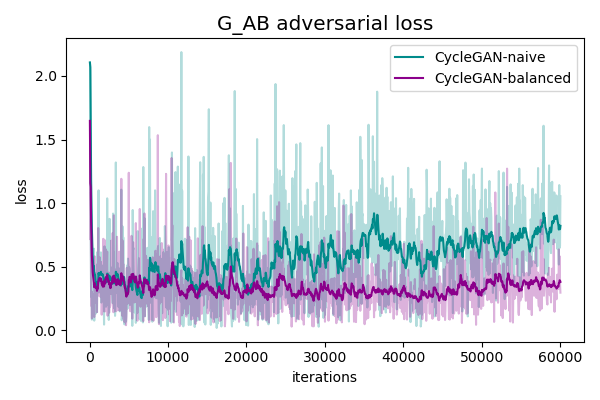
\includegraphics[width=.95\linewidth]{figures/Expt_2/gan_convergence/loss_G_AB.png}
        \caption{}
        \label{fig:loss_G_AB}
    \end{subfigure}
    \begin{subfigure}{.5\textwidth}
        \centering
        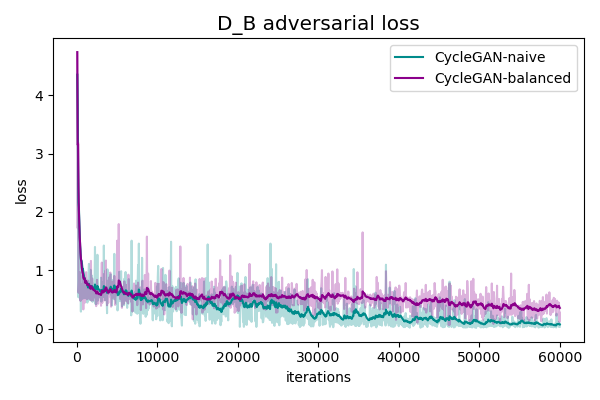
\includegraphics[width=.95\linewidth]{figures/Expt_2/gan_convergence/loss_D_B.png}
        \caption{}
        \label{fig:loss_D_B}
    \end{subfigure}
    \newline

    \begin{subfigure}{.5\textwidth}
        \centering
        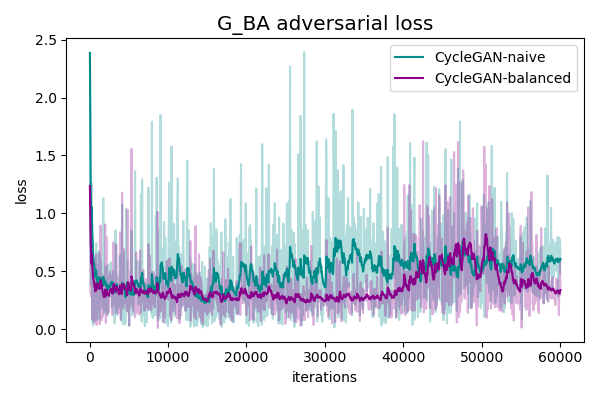
\includegraphics[width=.95\linewidth]{figures/Expt_2/gan_convergence/loss_G_BA.png}
        \caption{}
        \label{fig:loss_G_BA}
    \end{subfigure}
    \begin{subfigure}{.5\textwidth}
        \centering
        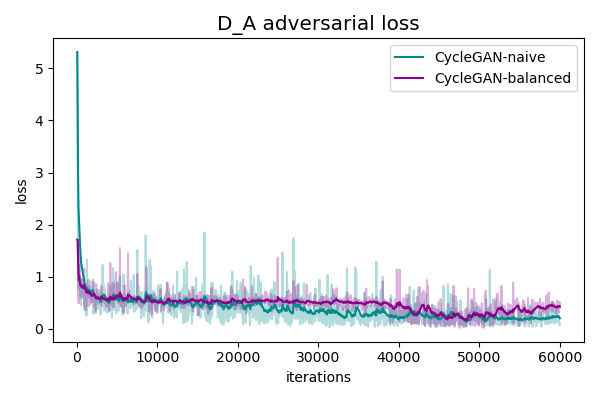
\includegraphics[width=.95\linewidth]{figures/Expt_2/gan_convergence/loss_D_A.png}
        \caption{}
        \label{fig:loss_D_A}
    \end{subfigure}
    
    \begin{subfigure}{.5\textwidth}
        \centering
        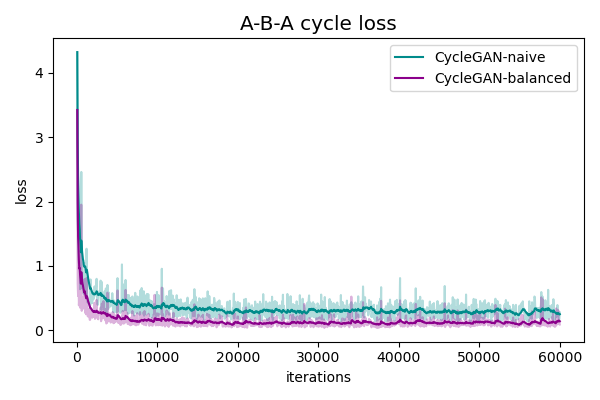
\includegraphics[width=.95\linewidth]{figures/Expt_2/gan_convergence/loss_cycle_A.png}
        \caption{}
        \label{fig:loss_cycle_A}
    \end{subfigure}
    \begin{subfigure}{.5\textwidth}
        \centering
        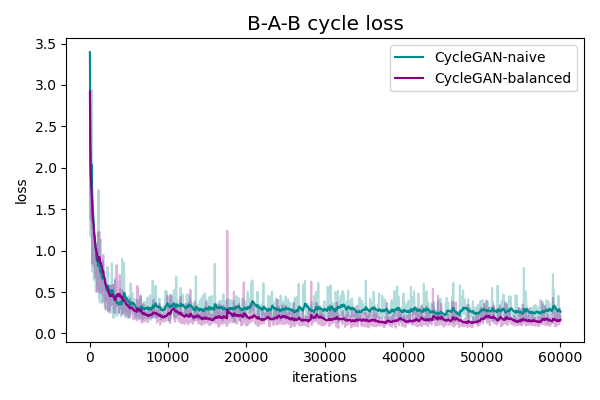
\includegraphics[width=.95\linewidth]{figures/Expt_2/gan_convergence/loss_cycle_B.png}
        \caption{}
        \label{fig:loss_cycle_B}
    \end{subfigure}

    \caption{Adversarial and cycle consistency loss curves for the two CycleGAN models. Exponential moving average smoothing was applied to each to show the general trend.}
    \label{fig:cyclegan_losses}
\end{figure}{}

Figure \ref{fig:cyclegan_losses} shows the adversarial training loss plots for CycleGAN-naive and CycleGAN-balanced. The aforementioned general reasoning is now applied independently to the two generator-discriminator pairs of the CycleGAN system. Consider the \textit{A}$\rightarrow$\textit{B} direction first. The adversarial loss $L({G_{AB})}$ of CycleGAN-balanced was closer to the equilibrium value than the that of CycleGAN-naive was, whose $G_{AB}$ was much more unstable and diverged away more significantly from around 25,000$^{th}$ iteration. This effect relates to the corresponding discriminator $D_B$ of CycleGAN-naive starting to overpower its $G_{AB}$ at around the same period. Discriminator $D_B$ of CycleGAN-balanced was maintained more stably around its equilibrium loss value of 0.5 over the full training period. Now looking at the \textit{B}$\rightarrow$\textit{A} direction, a similar pattern is observed. Except here, the generator-discriminator pair $G_{BA}$ and $D_A$ of CycleGAN-balanced appeared to destabilize and deviate away between 40,000$^{th}$ and 50,000$^{th}$ iteration, although eventually regaining stability near the end of the training. 

Additionally, cycle-consistency in CycleGAN-balanced was maintained to a greater extent almost throughout the training period as compared to CycleGAN-naive. The desirable training characteristics shown by the CycleGAN-balanced system can be attributed to its design modification.

\begin{figure}[h!]
    \makebox[\textwidth][c]
    {
        \begin{subfigure}{.4\textwidth}
            \centering
            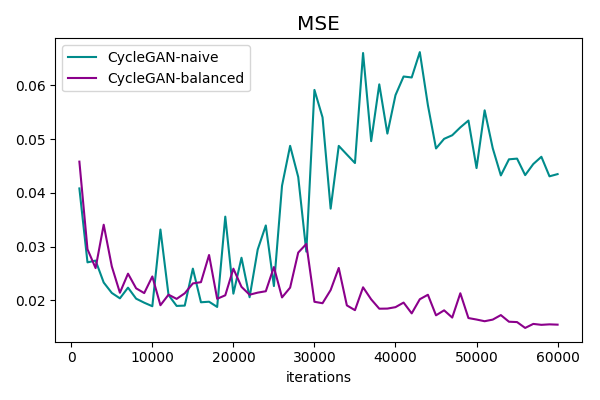
\includegraphics[width=\linewidth]{figures/Expt_2/gan_convergence/metric_val_mse.png}
            \caption{}
            \label{fig:metric_val_mse}
        \end{subfigure}
        \begin{subfigure}{.4\textwidth}
            \centering
            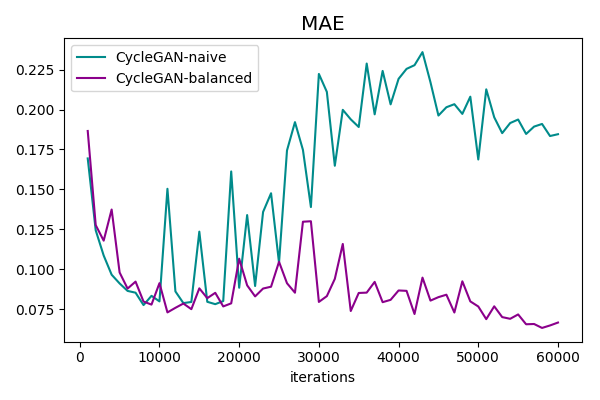
\includegraphics[width=\linewidth]{figures/Expt_2/gan_convergence/metric_val_mae.png}
            \caption{}
            \label{fig:metric_val_mae}
        \end{subfigure}
        \begin{subfigure}{.4\textwidth}
            \centering
            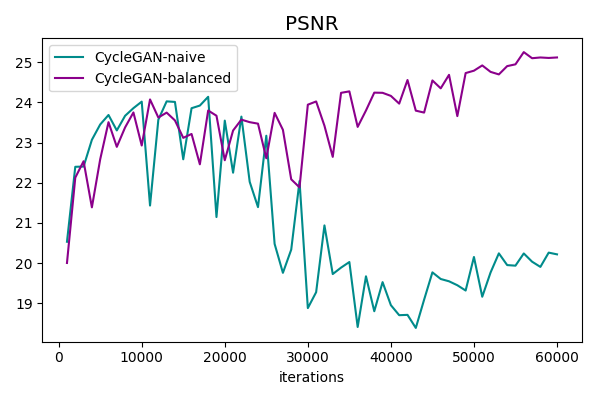
\includegraphics[width=\linewidth]{figures/Expt_2/gan_convergence/metric_val_psnr.png}
            \caption{}
            \label{fig:metric_val_psnr}
        \end{subfigure}
    }
    \newline
    \makebox[\textwidth][c]
    {
        \begin{subfigure}{.4\textwidth}
            \centering
            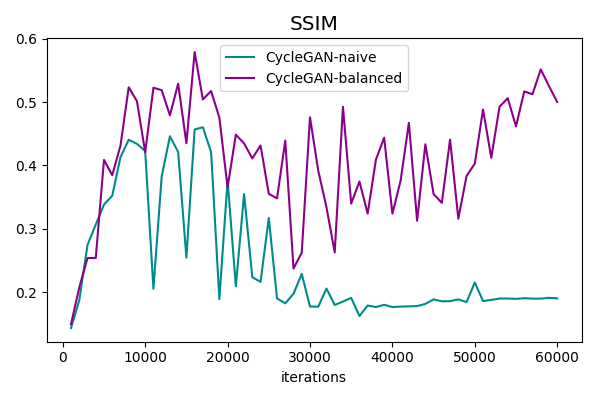
\includegraphics[width=\linewidth]{figures/Expt_2/gan_convergence/metric_val_ssim.png}
            \caption{}
            \label{fig:metric_val_ssim}
        \end{subfigure}
        \begin{subfigure}{.4\textwidth}
            \centering
            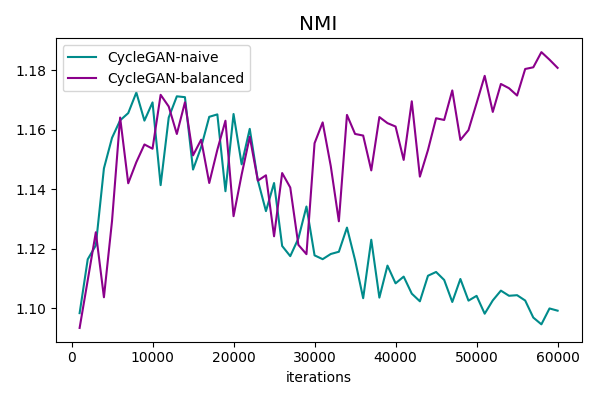
\includegraphics[width=\linewidth]{figures/Expt_2/gan_convergence/metric_val_nmi.png}
            \caption{}
            \label{fig:metric_val_nmi}
        \end{subfigure}
        \begin{subfigure}{.4\textwidth}
            \centering
            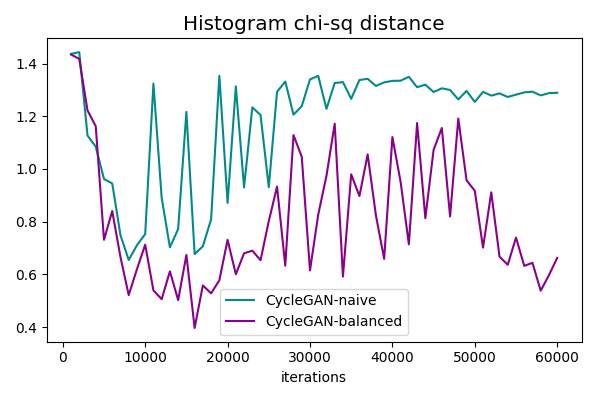
\includegraphics[width=\linewidth]{figures/Expt_2/gan_convergence/metric_val_histogram_chi2.png}
            \caption{}
            \label{fig:metric_val_histogram_chi2}
        \end{subfigure}
    }
    \caption{Validation metrics for the two CycleGAN models over the training period.}
    \label{fig:cyclegan_metrics}
\end{figure}{}

\subsubsection{Generalization performance} 
Next, we examine whether the same trend as was observed in the training convergence parameters is reflected in the models' generalization performance on the validation set. Figure \ref{fig:cyclegan_metrics} plots the six validation metrics for the CycleGAN models over the training period. The voxel-wise difference metrics -- MSE, MAE and PSNR -- show a generally consistent improvement in CycleGAN-balanced reflecting its relatively stable training. However, the metrics based on image intensity statistics -- SSIM, NMI and histogram $\chi^2$ distance -- show a brief, yet prominent, performance dip in the model halfway into the training suggesting a temporary drop in its generalizability. CycleGAN-naive followed a generally similar trend as CycleGAN-balanced up until approximately 25,000$^{th}$ iteration -- i.e. gradual improvement in the beginning followed by a performance dip. Though, contrary to CycleGAN-balanced, it was unable to recover its generalizability and continued to worsen. This correlates with the significant instability and divergence of the CycleGAN-naive model observed in the training convergence parameters at about the same period in the training process.

In summary, the image quality metrics applied on validation data were indeed informative about model convergence. Additionally, since some of them measured different properties of the generated images, they can be helpful in effectively tracking model generalizability.



%%%%%%%%%%%%%%%%%%%%%%%%%%%%%%%%%%%%%%%%%%%%%%%%%%%%%%%%%%%%%%%%%%%%%%%%%%%%%%%%%%%%%%%%%%%%%%%%%%%%%%%%%%%%%%%%%%%%%%%%%%%%%%%%%%%%%%%%%%%%%%%
\section{Experiment 3: Application-specific Downstream Tasks}
\label{Expt_3}
This experiment focuses on clinical evaluation of the synthetic hypoxia PET images by quantifying hypoxia inside the gross tumor volume (GTV).


% ---------------------------
\subsection{Experiment Setup}
HX4-PET-syn images are computed for each patient in the validation set using the fully trained models, their units converted to SUV scale, and stored as NRRD files. The images are then loaded and analyzed. Each HX4-PET-syn image and its corresponding ground truth HX4-PET-reg are first cropped to a bounding box containing just the GTV. The GTV mask is then applied to the images, and intensities outside the mask are set to 0. Next, the GTV SUV values are converted to the tumor-to-background ratio (TBR) by dividing each GTV voxel's SUV with $SUV_{aorta-mean}$. From this point onward, the different hypoxia quantification metrics are computed separately as follows:

\begin{enumerate}
    
    \item \textit{MSE-GTV and SSIM-GTV:} MSE and SSIM are calculated only on the GTV voxels using array masking.
    
    \item \textit{Hypoxic tumor classification:} One of the ways of classifying the tumor as hypoxic or non-hypoxic is by calculating the total physical volume of the hypoxic region in the GTV, known as hypoxic volume (HV), and applying a threshold. We calculate HV by first performing point-wise intensity thresholding using standard TBR threshold of 1.4 (Zegers et al. \cite{zegers2013hypoxia}) to obtain a binary image of hypoxic voxels followed by calculating the total physical volume (in mm$^3$) occupied by them. Then, HV threshold of 1 cm$^3$ is applied beyond which the tumor is classified as hypoxic, similar to Even et al. \cite{even2017predicting}. Tumor classification is performed for each predicted image and its corresponding ground truth, and the mean accuracy is derived.
    
    \item \textit{Hypoxic region segmentation:} The 3D hypoxic region in the GTV is segmented by applying the standard TBR threshold of 1.4. This is performed for each predicted image and its corresponding ground truth image. Then, the Dice Similarity Coefficient (DSC) is used to measure the overlap between the hypoxic regions. 

\end{enumerate}


% -------------------------------
\subsection{Results and Analysis}
Table \ref{tab:hypoxia_metrics} reports the mean values of the hypoxia quantification measures over the validation set. The quantitative results provide no conclusive evidence on the model performances and are, in fact, slightly contradictory to previous results. MSE-GTV and SSIM-GTV were very similar for all the models, and Pix2Pix was less competent in accurately predicting the hypoxic regions. CycleGAN-balanced didn't show an improvement over CycleGAN-naive here. A visualization of the predicted tumor hypoxia patterns is shown in Figure \ref{fig:hypoxia_viz}. Two important observations can be made are. First, the Pix2Pix outputs show significant checkerboard-like noise patterns. Note that these are of different nature compared the image-wide foreground noise defined as a failure criterion earlier in experiment \ref{Expt_2} in that these are of higher frequency and are localized to high-intensity regions, such as the tumor locality shown in the figure. Predictions from the CycleGANs show minimal noise. Second, Pix2Pix predictions do not contain sufficiently high intensity regions to be capable of being segmented and their spatial patterns do not match the hypoxic patterns in the ground truth. Since only a small number of voxels carry sufficiently high intensity values, there existed many false-negative voxels which collectively amounted to hypoxic tumors being misclassified as non-hypoxic. In case of the CycleGANs, their predicted hypoxic patterns are more similar to the metabolic patterns from FDG-PET, instead of the ground truth.

% % Original table
% \begin{table}[h!]
%     \footnotesize
%     \centering
%     \makebox[\textwidth][c]
%     {
%         \begin{tabular}{ccccc}
%             \textbf{Method}   & \textbf{MSE-GTV}   & \textbf{SSIM-GTV}   & \textbf{Tumor classif. acc.}   & \textbf{Hypoxic region seg. Dice} \\
%             \hline
%             Pix2Pix   & \textbf{0.067} $\pm$ 0.040   & 0.870 $\pm$ 0.082   & 61.2\% (12/19)   & 0.058 $\pm$ 0.092 \\
%             CycleGAN-naive   & 0.079 $\pm$ 0.046   & \textit{0.884} $\pm$ 0.066   & \textbf{78.9}\% (15/19)   & \textbf{0.141} $\pm$ 0.184 \\
%             CycleGAN-balanced   & \textit{0.068} $\pm$ 0.042   & \textbf{0.886} $\pm$ 0.066   & \textit{73.7\%} (14/19)   & \textit{0.127} $\pm$ 0.174 \\
%         \end{tabular}
%     }
%     \caption{Results of tumor hypoxia quantification. Best and second-to-best values are highlighted with bold and italics font, respectively. For tumor classification, the accuracy is given in percentage values and fraction of patients with correctly classified tumors.}
%     \label{tab:hypoxia_metrics}
% \end{table}

% Transposed table
\begin{table}[h!]
    \footnotesize
    \centering
    \begin{tabular}{l || lll}
         \textbf{Method} $\rightarrow$                & Pix2Pix                       & CycleGAN-naive                & CycleGAN-balanced              \\
         \hline
         \textbf{MSE-GTV}                             & \textbf{0.067} $\pm$ 0.040    & 0.079 $\pm$ 0.046             & \textit{0.068} $\pm$ 0.042     \\
         \textbf{SSIM-GTV}                            & 0.870 $\pm$ 0.082             & \textit{0.884} $\pm$ 0.066    & \textbf{0.886} $\pm$ 0.066     \\
         \textbf{Tumor classification accuracy}       & 61.2\% (12/19)                & \textbf{78.9}\% (15/19)       & \textit{73.7\%} (14/19)        \\
         \textbf{Hypoxic region seg. Dice}    & 0.058 $\pm$ 0.092             & \textbf{0.141} $\pm$ 0.184    &  \textit{0.127} $\pm$ 0.174    \\
    \end{tabular}
    \caption{Results of tumor hypoxia quantification. Best and second-to-best values are highlighted with bold and italics font, respectively. For tumor classification, the accuracy is given in percentage values and fraction of patients with correctly classified tumors.}
    \label{tab:hypoxia_metrics}
\end{table}



\begin{figure}[h!]
    \centering
    \makebox[\textwidth][c]
    {
        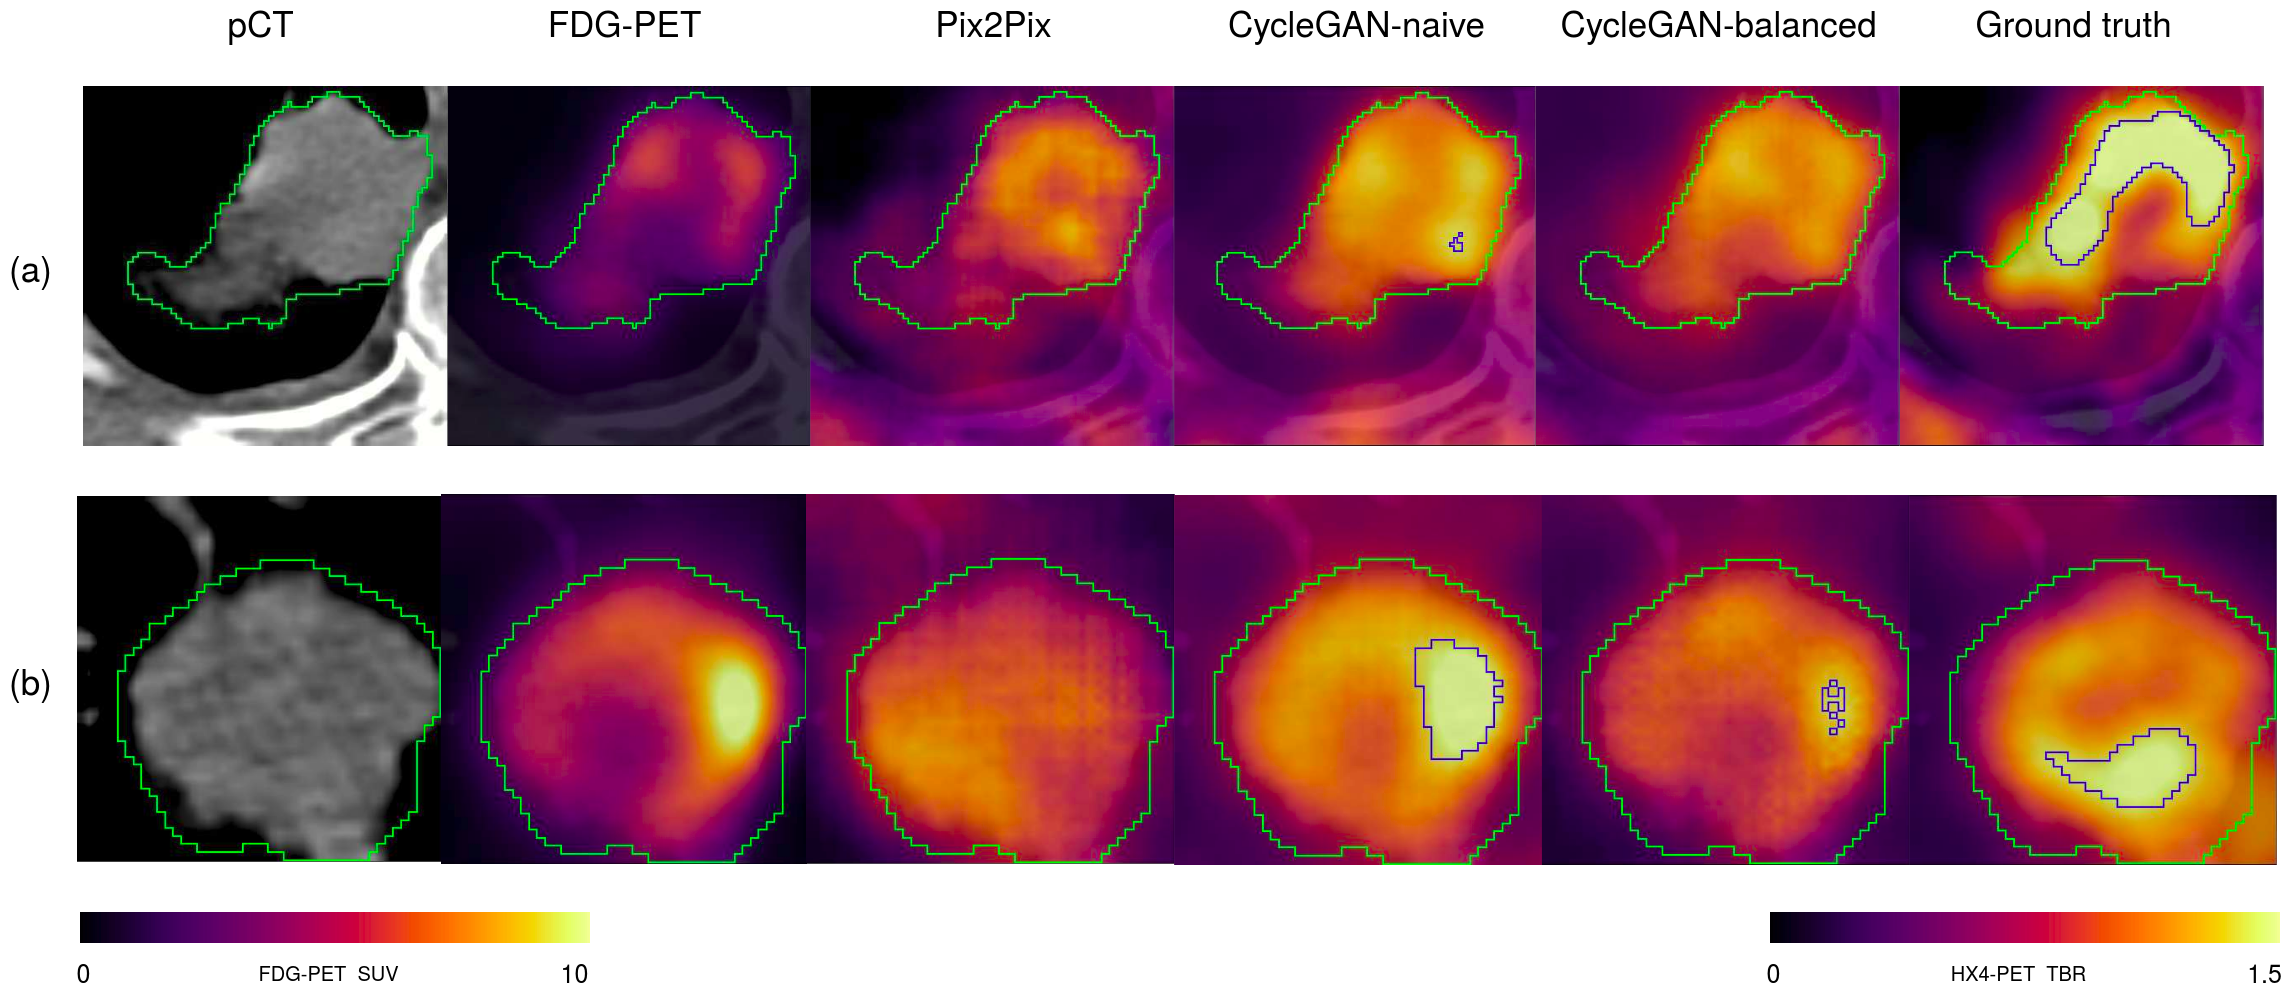
\includegraphics[width=\linewidth]{figures/Expt_3/hypoxia_viz.png}
    }
    \caption{Tumor hypoxia patterns generated by the models. GTV is delineated with green contour, and the hypoxic region in each of three models' prediction and the ground truth is marked with blue contours. In both examples, Pix2Pix predictions didn't contain sufficiently intense regions, hence no hypoxic areas are seen segmented in these slices.}
    \label{fig:hypoxia_viz}
\end{figure}

One of the reasons Pix2Pix fails here appears to be related to its supervised training. The ground truth images contain registration errors that are more pronounced at the small scale in which this evaluation is performed. The fine hypoxia patterns in the ground truth, including those within the tumor, might have shifted post-registration causing misalignment with the CT and FDG-PET features, thereby inducing noise in the paired training data. Therefore, although the Pix2Pix model could produce synthetic hypoxia images of an overall higher quality, these images reveal large inaccuracies when examined at the scale of the tumor.
In case of the two CycleGANs, the tumor hypoxia patterns matched the spatial pattern of FDG uptake suggesting that the models learned to excessively depend on FDG-PET features. Another reason for poor clinical performance of all three models might be the small size of the training dataset. Even when using a patch-based training approach, the number of sufficiently varied training samples was very low. Training on a larger dataset could likely improve performance.
